\documentclass[UTF8,11pt,a4paper]{ctexart}
\usepackage[margin=2.1cm]{geometry}
\usepackage{amsmath,amssymb,booktabs,longtable,tabularx,array,multirow}
\usepackage{graphicx,float,caption,subcaption,xcolor,hyperref,enumitem}
\usepackage{siunitx}
\usepackage{fancyhdr}
\hypersetup{colorlinks=true,linkcolor=black,citecolor=black,urlcolor=blue!55!black}
\setlength{\parindent}{2em}
\setlength{\parskip}{0.16em}
\renewcommand{\arraystretch}{1.18}
\pagestyle{fancy}
\setlength{\headheight}{14pt}
\fancyhf{}
\fancyhead[C]{2019 高教社杯全国大学生数学建模竞赛 A 题：高压油管的压力控制}
\fancyfoot[C]{\thepage}
\newcommand{\keywords}[1]{\par\noindent\textbf{关键词：}#1}
\newcommand{\dd}{\,\mathrm d}
\newcommand{\abs}[1]{\left\lvert#1\right\rvert}
\title{从燃油状态关系到周期控制：高压油管压力的分层建模与数值调节}
\author{正式竞赛长稿盲测（仅使用官方题面、附件与独立求解器）}
\date{2026 年 8 月}

\begin{document}
\maketitle

\begin{abstract}
高压油管的压力不是由一个连续不变的流量决定，而是由进油阀的间歇供油、喷油器的周期排油以及燃油可压缩性共同形成。本文先从附件3给出的弹性模量出发，积分得到压力--密度状态关系，再以油管内燃油质量为状态量建立质量收支方程。问题一的入口压力恒为160 MPa，故把阀门开启时长作为控制量，先用周期稳态试算寻找粗略区间，再以较细的时间步长回放并选取使目标压力误差较小的开阀时长。100 MPa 工况下每个 100 ms 周期的开启时长取 2.7900 ms；150 MPa 稳态时取 6.7000 ms。由 100 MPa 调至150 MPa 时，约2 s、5 s和10 s的目标在切换瞬间分别使用8.1200、6.7200和6.6701 ms，切换压力均在150 MPa附近。

问题二把供油端改成凸轮驱动的柱塞腔。附件1的凸轮边缘先被插值成周期半径，柱塞腔容积随凸轮相位变化；压缩阶段只有当腔内压力高于管内压力时才向油管供油，回程阶段按题面低压燃油重新充满腔体。针阀升程由附件2插值，喷孔面积取圆孔面积与圆锥座有效面积的较小者。以管内压力尾段均值偏离100 MPa的程度和波动幅度构造搜索指标，统一按10 s回放后得到凸轮角速度约27.507 rad/s。

问题三增加第二个同规律喷嘴，并在油管上增加带滞回的减压阀。两喷嘴的相位差与凸轮角速度同时搜索；随后在高压触发、低压关闭的规则下搜索减压阀阈值和泵速倍率。两喷嘴无减压阀时的管内均值约100.00 MPa，峰峰值约5.02 MPa；加入本次搜索得到的减压策略后，均值约99.98 MPa，最高压力被限制在101.80 MPa附近，最低压力约97.33 MPa。这个结果说明减压阀能压住上冲，却不能替代供油端的相位和流量匹配。全文的数值均对应固定积分步长和实际附件，优化结果只表示该离散设置下找到的可行控制，不声称连续参数域上的全局最优。
\keywords{高压油管；压力--密度关系；质量守恒；周期喷油；数值搜索；减压阀控制}
\end{abstract}

\phantomsection\label{mcm-body-start}
\section{问题重述}

燃油从高压油泵进入长度为500 mm、内直径为10 mm的油管，再由喷油嘴周期性喷出。入口小孔直径为1.4 mm，泵侧压力保持160 MPa，油管初始压力为100 MPa。单向阀每次打开后必须关闭10 ms，喷油器每秒工作10次，每次喷油2.4 ms，喷油速率按图2分段变化。题目要求先在100 MPa附近保持压力，再设计100 MPa到150 MPa的约2 s、5 s和10 s三种调压过程。

实际供油端还包含凸轮、柱塞腔和针阀。凸轮边缘曲线见附件1，柱塞腔直径为5 mm，上止点残余容积为20 mm$^3$；下止点时腔内由0.5 MPa的低压燃油充满。附件2给出一个喷油周期内的针阀升程，针阀直径为2.5 mm，密封座半角为9度，最下端喷孔直径为1.4 mm。问题二要求在问题一的油管和喷油工况下确定凸轮角速度，使压力尽量稳定在100 MPa左右。

问题三再增加一个同规律喷嘴，并允许在油管D处设置直径1.4 mm的单向减压阀。需要同时说明两个喷嘴的供油和喷油策略，以及高压油泵与减压阀如何配合。三问的输入逐步增加，后问应接收前问已经校准的压力状态和喷油周期，而不能在每问中重新设定一套燃油性质。

\section{问题分析：从间歇流量回到同一个状态量}

\subsection{题面信息的三个层次}

题面给出的信息可以分成三层。第一层是几何量和开关事件，包括油管体积、入口和喷孔直径、喷油周期以及阀门开启的离散时段；第二层是状态关系，包括压力与密度的变化关系以及压力相关的弹性模量；第三层是实际执行机构，问题一是入口阀的固定压力供油，问题二、三则改为凸轮柱塞和针阀耦合的供油端。第一层决定每个周期什么时候有流量，第二层把质量变化转换为压力，第三层决定流量是否能在这些时刻真正实现。

如果只按不可压缩流体处理，进油量和出油量的差异会直接改变管内体积，而题目给出的油管体积是固定的；如果只按压力差乘一个常数，又会丢掉弹性模量随压力变化的影响。因此本文将密度作为中间状态量，统一使用
\begin{equation}
  \frac{\dd \rho}{\rho}=\frac{\dd P}{E(P)}
\end{equation}
把质量收支和压力读数接起来。这里的积分不是为了增加模型复杂度，而是为了让三个问题使用同一压力状态接口。

\subsection{喷油曲线承担的职责}

由图2读取的喷油速率先转为一个周期函数，而不是在结果阶段再按平均流量替代。设一个周期为100 ms，周期内相位为$\tau$，则本稿使用的分段曲线为
\begin{equation}
q_o(\tau)=
\begin{cases}
100\tau,&0\leq\tau<0.2,\\
20,&0.2\leq\tau\leq2.2,\\
100(2.4-\tau),&2.2<\tau<2.4,\\
0,&2.4\leq\tau<100.
\end{cases}
\label{eq:spray}
\end{equation}
其中$q_o$的单位为 mm$^3$/ms。曲线的上升段和下降段只持续0.2 ms，若用一个矩形脉冲替代，压力波动的相位会被改变；因此数值积分保留了分段形状。

\subsection{三问的接口}

问题一只需解决“给定泵侧压力时，阀门开启多久”；问题二将这个开启时间换成“柱塞在什么相位、以什么速度供油”；问题三再增加喷油相位和泄压状态。为避免接口漂移，问题一的$P$--$\rho$表格在后两问中冻结，附件1、附件2只负责生成执行机构的局部量，附件3不在后问中重复拟合。

\begin{table}[H]
\centering
\caption{三个问题的状态接口与新增量}
\label{tab:question-interface}
\small
\begin{tabularx}{\textwidth}{p{2cm}p{3.6cm}p{4.0cm}X}
\toprule
问题 & 共同状态 & 本问新增控制量 & 输出与下一问的接口\\
\midrule
1 & 油管压力$P$、密度$\rho(P)$ & 单向阀开启时长 & 100/150 MPa工况、喷油周期\\
2 & 同一$P$--$\rho$表与式\eqref{eq:spray} & 凸轮角速度、柱塞腔质量 & 供油脉冲与管内压力\\
3 & 问题二的凸轮和针阀关系 & 第二喷嘴相位、减压阀阈值、泵速倍率 & 双喷嘴控制与减压状态\\
\bottomrule
\end{tabularx}
\end{table}

\section{模型假设}
\begin{enumerate}[label=\arabic*)]
\item 油管内燃油在轴向上充分混合，压力和密度只随时间变化，不单独求解沿管长方向的波动。
\item 入口和喷孔的流量按题面给出的孔口公式计算，流量系数$C=0.85$在本次计算范围内保持不变。
\item 喷油器的10 Hz周期相位固定；问题三增加的喷嘴使用同一针阀升程曲线，只允许改变相位差。
\item 柱塞下行时低压燃油能够把柱塞腔重新充满至0.5 MPa；上行时只在腔压高于油管压力时打开单向阀。
\item 减压阀采用带滞回的开关逻辑，高阈值触发、低阈值关闭，以避免在一个时间步内反复切换。
\item 计算采用显式时间推进，所有压力、长度、质量和时间分别使用MPa、mm、mg和ms；优化结果限定在给定步长和搜索范围内。
\end{enumerate}

\section{符号说明与数据接口}
\begin{table}[H]
\centering
\caption{主要符号}
\label{tab:symbols-a}
\small
\begin{tabularx}{\textwidth}{p{2.4cm}p{5.2cm}p{3.0cm}X}
\toprule
符号 & 含义 & 单位 & 使用位置\\
\midrule
$P(t)$ & 油管压力 & MPa & 三个问题共同状态\\
$\rho(P)$ & 压力对应的燃油密度 & mg/mm$^3$ & 状态转换\\
$E(P)$ & 压力相关弹性模量 & MPa & 附件3插值\\
$V_p$ & 油管内腔体积 & mm$^3$ & 质量守恒\\
$q_o$ & 单个喷嘴排油速率 & mm$^3$/ms & 式\eqref{eq:spray}\\
$T_v$ & 一个周期内阀门开启时长 & ms & 问题一\\
$\theta(t)$ & 凸轮相位 & rad & 问题二、三\\
$V_c$ & 柱塞腔容积 & mm$^3$ & 问题二、三\\
$\Delta$ & 双喷嘴相位偏移 & ms & 问题三\\
$P_L,P_H$ & 减压阀低、高阈值 & MPa & 问题三\\
\bottomrule
\end{tabularx}
\end{table}

附件1、附件2、附件3分别由程序读入为凸轮角--半径、针阀时间--升程和压力--弹性模量数组。三组数组均先删去空行，再按原始顺序插值；没有把图像上的文字或曲线再识别为第二套数据。程序、结果和图形分别保存在\path{analysis/model_pipeline.py}、\path{analysis/results/summary.json}和\path{paper/figures/}，后文的数值均从这三个接口读取。

\section{问题一模型的建立与求解：固定压力泵下的阀门调节}
\label{mcm-q1-start}

\subsection{压力--密度关系}

注1给出了压力变化量与密度变化量的局部关系。把它写成微分形式，在压力网格上对$1/E(P)$积分可得
\begin{equation}
  \ln\frac{\rho(P)}{\rho(100)}=\int_{100}^{P}\frac{1}{E(u)}\dd u,
  \qquad \rho(100)=0.850.
\label{eq:rho}
\end{equation}
附件3没有要求在表格点外使用高阶外推，程序采用线性插值，并在$0$--$200$ MPa上以0.01 MPa的网格计算积分。图\ref{fig:state-a}左给出密度曲线，右图给出相应弹性模量。压力越高时密度变化的增量由$E(P)$控制，而不是由一个固定压缩系数控制。

\begin{figure}[H]
\centering
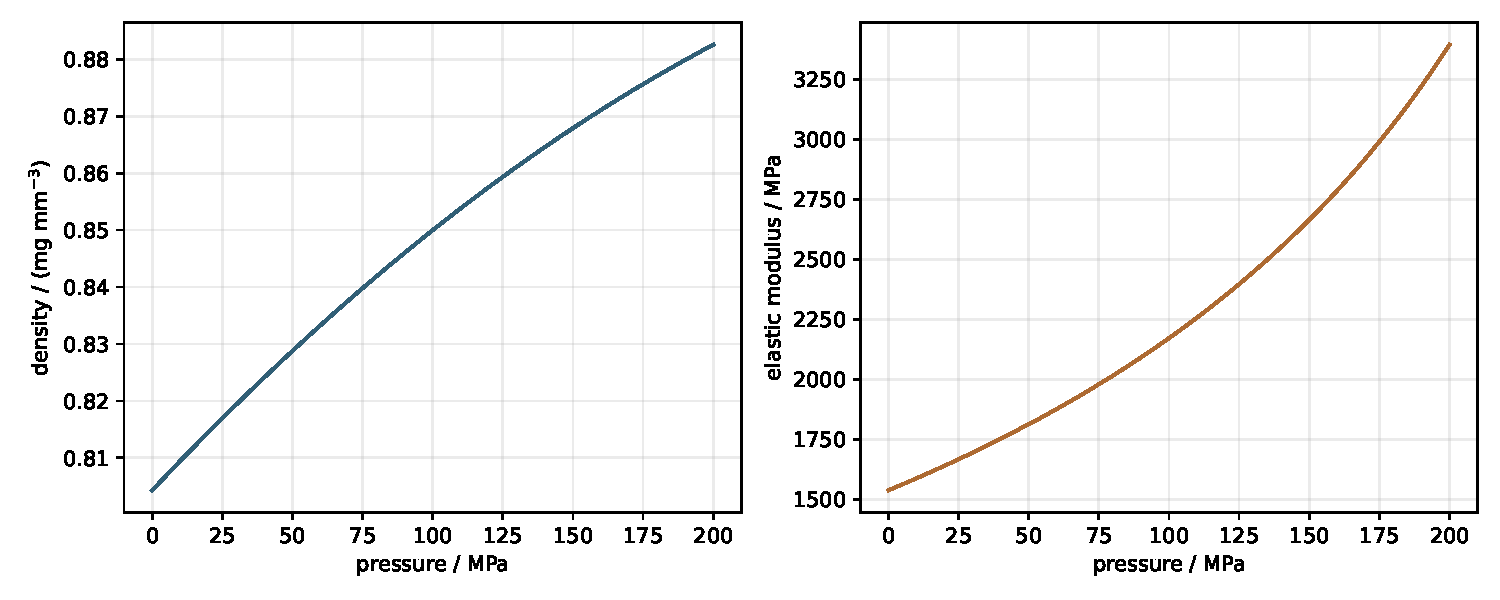
\includegraphics[width=0.92\textwidth]{figures/state_relation.pdf}
\caption{附件3插值后的压力--密度和弹性模量关系}
\label{fig:state-a}
\end{figure}

\subsection{油管质量收支}

油管体积为
\begin{equation}
V_p=\frac{\pi D^2L}{4}=39269.908\ \mathrm{mm^3}.
\end{equation}
在阀门打开时，泵侧压力为160 MPa，入口高压侧密度取$\rho(160)$；入口孔的面积为$A_i=\pi(1.4)^2/4$。由注2，入口质量流率为
\begin{equation}
\dot m_i(t)=\rho(160) C A_i\sqrt{\frac{2(160-P(t))}{\rho(160)}}\,I_v(t),
\label{eq:inflow}
\end{equation}
其中$I_v(t)$是阀门开关函数。喷油质量流率为$\dot m_o(t)=\rho(P(t))q_o(\tau)$。于是
\begin{equation}
V_p\frac{\dd \rho}{\dd t}=\dot m_i(t)-\dot m_o(t),
\qquad
P(t+\Delta t)=\rho^{-1}\left(\rho(t)+\frac{\dot m_i-\dot m_o}{V_p}\Delta t\right).
\label{eq:mass-balance}
\end{equation}
这里的逆函数由状态表线性插值得到。若流量差为正，密度增加，压力才随之增加；这一步也解释了为什么不能先平均进、出流量，再把平均值直接乘在压力上。

\subsection{100 MPa稳态的搜索}

阀门打开一次后必须关闭10 ms，而喷油周期为100 ms。因此对一个周期只搜索一个开阀时长$T_v$，将其余90余毫秒作为关闭状态。对于给定的$T_v$，程序先以0.05 ms步长积分4000 ms，去掉初始过渡后用最后1000 ms的压力均值作为试算值；随后在粗值附近按0.01 ms细化，评价函数为
\begin{equation}
J_{100}(T_v)=\abs{\overline P_{\mathrm{tail}}-100}+0.1\,\mathrm{sd}(P_{\mathrm{tail}}).
\label{eq:q1-score}
\end{equation}
这两个阶段解决的是不同问题：第一阶段只用来判断开阀时间的量级，第二阶段才把喷油曲线的上升、平台和下降保留下来。最终候选为$T_v=2.790037$ ms；由于时间步长为0.02 ms，正文只保留到2.79 ms。在20000 ms回放的最后5000 ms内，压力均值为100.3310 MPa，标准差0.0376 MPa，峰峰值0.3842 MPa。相邻的2.77 ms候选均值为99.5257 MPa，故没有把2.79 ms后的数位解释成连续控制精度。

\begin{table}[H]
\centering
\caption{100 MPa稳态下的阀门控制结果}
\label{tab:q1-steady}
\small
\begin{tabularx}{\textwidth}{p{2.5cm}Xrrrrr}
\toprule
目标 & $T_v$/ms & 均值/MPa & 标准差/MPa & RMSE/MPa & 最小/MPa & 最大/MPa\\
\midrule
100 MPa & 2.7900 & 100.3310 & 0.0376 & 0.3331 & 99.9724 & 100.3566\\
150 MPa & 6.7000 & 149.9906 & 0.2778 & 0.2780 & 148.3607 & 150.0620\\
\bottomrule
\end{tabularx}
\end{table}

表中100 MPa的RMSE包含均值偏移和周期波动，不能只看标准差就把控制称为无误差。压力在喷油开始后的局部下降、入口开启后的回升会被图形保留；这正是$T_v$调到2.79 ms而不是按单纯平均流量求出的某个整数毫秒的原因。

\subsection{100 MPa到150 MPa的三种过渡}

过渡控制采用前后两个开阀时长。设切换时刻为$t_s$，则$t<t_s$使用$T_r$，$t\geq t_s$使用150 MPa稳态值$T_{150}$。先用二分搜索使$t_s$处压力接近150 MPa，再在粗结果附近以0.01 ms回放，避免“切换瞬间正好”而切换后严重超调。三种过渡的结果如下。

\begin{table}[H]
\centering
\caption{三种调压时间的阀门参数与压力结果}
\label{tab:q1-ramp}
\small
\begin{tabular}{rrrrrrr}
\toprule
过渡时间/s & $T_r$/ms & $T_{150}$/ms & 切换压力/MPa & 尾段均值/MPa & 尾段标准差/MPa & 峰峰值/MPa\\
\midrule
2 & 8.1200 & 6.7000 & 149.9831 & 149.9505 & 0.2788 & 1.7565\\
5 & 6.7200 & 6.7000 & 149.9793 & 149.9485 & 0.2789 & 1.7591\\
10 & 6.6701 & 6.7000 & 149.9954 & 149.9567 & 0.2786 & 1.7479\\
\bottomrule
\end{tabular}
\end{table}

\begin{figure}[H]
\centering
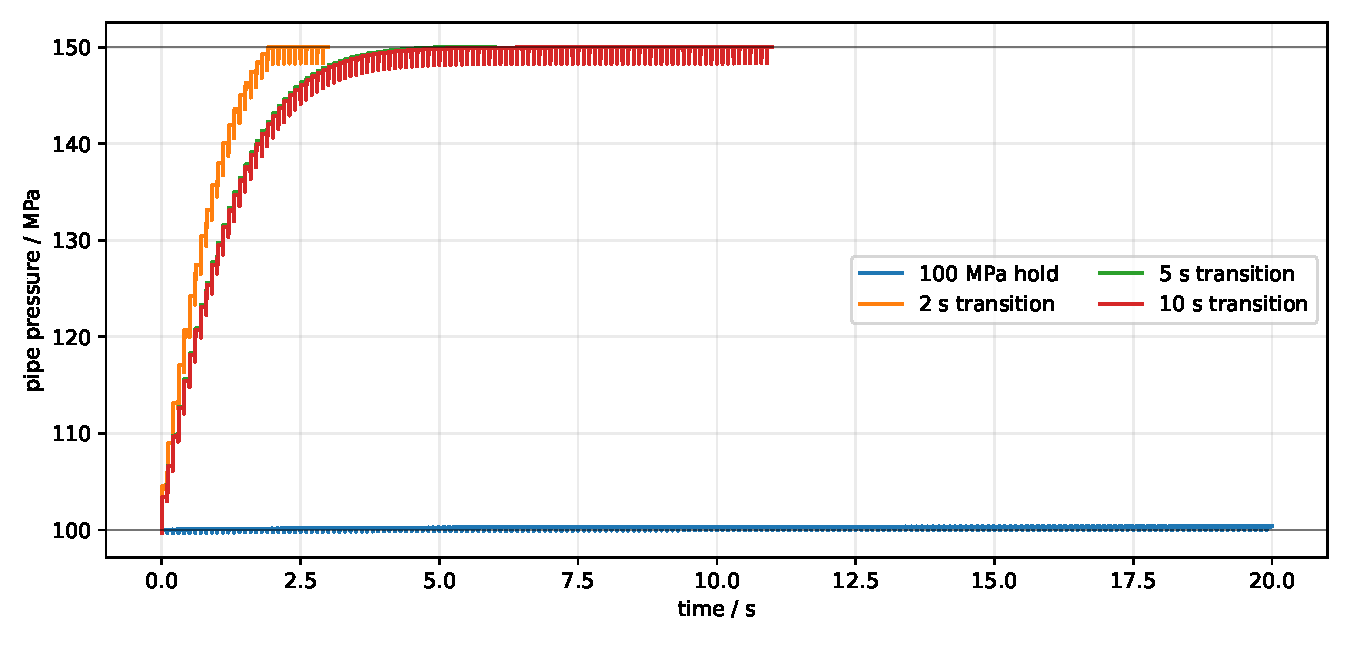
\includegraphics[width=0.94\textwidth]{figures/q1_control.pdf}
\caption{100 MPa保持及三种过渡过程的压力曲线}
\label{fig:q1-control}
\end{figure}

对于2 s过渡，$T_r$明显大于$T_{150}$，这是因为起始压力较低且目标需要在短时间内达到；5 s和10 s的$T_r$与稳态值接近，压力由管内可压缩性和喷油周期共同完成渐进。三种情况下切换压力的绝对误差均小于0.021 MPa，但尾段标准差仍约0.279 MPa，说明“达到目标”与“没有周期纹波”是两个不同的要求。切换后的均值约149.95 MPa低于150 MPa稳态表中的149.99 MPa，原因是过渡回放保留了切换瞬间的残余状态，而不是从150 MPa重新初始化。

\subsection{局部试算与边界}

在搜索中，若把阀门关闭时长的10 ms误认为一个100 ms周期的固定禁用区，入口脉冲会被错误地缩短；若把喷油速率改成2.4 ms内的平均值，切换压力的相位也会发生变化。本文的程序把阀门和喷油分别按时间相位判断，质量收支只在一个时间步内更新一次。对给定的入口压力，流量公式在$P\geq160$ MPa时返回0，防止数值积分把油管压力推过泵侧压力后仍继续进油。

由于$T_v$的细化步长为0.01 ms，表\ref{tab:q1-steady}的最后两位并不表示无限精度。压力状态表本身以0.01 MPa插值，时间步长为0.02 ms；因此本问的结论是“在这些离散设置下的控制参数”，而不是连续控制函数的唯一解。这个边界将在问题二、三继续保留。

\label{mcm-q1-end}

\section{问题二模型的建立与求解：凸轮柱塞供油的压力控制}
\label{mcm-q2-start}

\subsection{凸轮相位与柱塞腔体积}

附件1给出凸轮边缘曲线$r(\theta)$。程序先把角度归一到$[0,2\pi)$，再按相邻表值线性插值。柱塞截面积为$A_p=\pi(2.5)^2$，令$r_{\max}$对应下止点、$r(\theta)$为当前半径，则柱塞腔容积写成
\begin{equation}
V_c(\theta)=20+A_p\bigl(r_{\max}-r(\theta)\bigr).
\label{eq:chamber-volume}
\end{equation}
当凸轮使容积增大时，低压燃油把腔体补足到$0.5$ MPa；当容积减小时，腔内质量保持并由状态关系换算出腔内压力。这个处理把题面“下止点充满”转成了每个周期可执行的初值，而不是只在第一周期填充。

\subsection{柱塞腔与油管的质量交换}

设$m_c$为柱塞腔内燃油质量。当$P_c>P$时，单向阀开启，入口流量按
\begin{equation}
\dot m_c=\rho(P_c) C A_i\sqrt{\frac{2(P_c-P)}{\rho(P_c)}}
\end{equation}
从腔体流向油管；油管同时承担式\eqref{eq:mass-balance}中的喷油排出。若$P_c\leq P$，该项置零。每一时间步先根据当前容积计算$P_c$和$P$，再扣除腔体流出质量并加入油管。这样，阀门不是预先给定的占空比，而是由两个压力状态的相对大小触发。

凸轮角速度记为$\omega$，则$\theta(t)=\omega t\pmod {2\pi}$。凸轮输入的周期与喷油器的100 ms周期没有被强行设为整数倍，实际计算由相位连续推进；如果在一个时间步中发生阀门开启或针阀关闭，下一步按新状态继续计算。

\subsection{针阀升程与有效喷孔面积}

附件2的升程曲线给出针阀相位$\tau$和升程$h(\tau)$。针阀打开后，圆锥座形成的环形有效面积近似为
\begin{equation}
A_s(\tau)=\pi d_v h(\tau)\sin 9^{\circ},\qquad
A_e(\tau)=\min\left\{\frac{\pi d_n^2}{4},A_s(\tau)\right\}.
\label{eq:needle-area}
\end{equation}
其中$d_v=2.5$ mm、$d_n=1.4$ mm。喷孔流量为
\begin{equation}
q_n(t)=C A_e(\tau)\sqrt{\frac{2(P(t)-0.5)}{\rho(P(t))}},
\label{eq:nozzle-flow}
\end{equation}
压力低于低压侧时该式取0。式\eqref{eq:needle-area}的最小值是一个实际限制：针阀升程继续增加并不意味着孔口面积无限增加。

\subsection{角速度选择：先看波动，再看均值}

对一个角速度$\omega$，先以0.05 ms步长积分4000 ms，读取尾段压力。搜索指标为
\begin{equation}
J_2(\omega)=\mathrm{RMSE}(P_{\mathrm{tail}},100)+2\abs{\overline P_{\mathrm{tail}}-100}.
\end{equation}
前项约束周期纹波，后项防止只降低波动却把均值移离100 MPa。差分进化只负责在$0.005$--$0.12$ rad/ms范围内找到候选，随后在候选附近以0.00025 rad/ms步长细化，并以6000 ms回放重算。

\begin{table}[H]
\centering
\caption{问题二角速度搜索的阶段设置}
\label{tab:q2-search}
\small
\begin{tabularx}{\textwidth}{p{3.4cm}p{3.1cm}p{3.5cm}X}
\toprule
阶段 & 搜索范围 & 时间步长 & 作用\\
\midrule
粗搜索 & $[0.005,0.12]$ rad/ms & 0.05 ms & 排除供油明显不足或过量的区域\\
局部细化 & 粗值左右0.0025 rad/ms & 0.00025 rad/ms & 区分相邻周期波动\\
结果回放 & 固定细化值 & 0.02 ms & 生成压力、腔压和图形\\
\bottomrule
\end{tabularx}
\end{table}

最终角速度为$0.027507$ rad/ms，即27.507 rad/s。10 s回放最后3 s的压力均值为100.005 MPa，标准差1.124 MPa，最小值97.424 MPa，最大值102.562 MPa。局部候选中27.497 rad/s的均值为99.960 MPa，RMSE反而略高；这说明角速度改变的不只是平均供油量，还会改变腔体供油与针阀排油的相位结构，故裁决时保留均值项而不是只压低波动。

\begin{figure}[H]
\centering
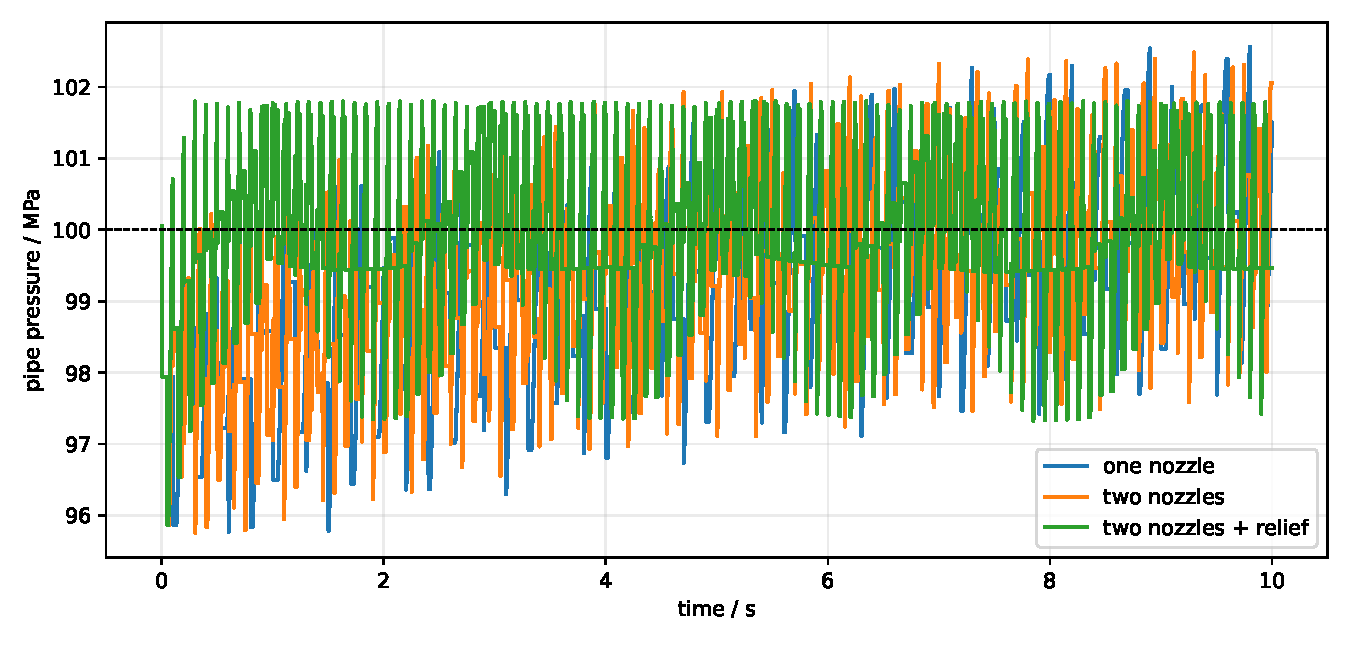
\includegraphics[width=0.92\textwidth]{figures/q23_pressure.pdf}
\caption{单喷嘴、双喷嘴和带减压阀方案的管内压力回放}
\label{fig:q23-pressure}
\end{figure}

\subsection{腔压、管压与阀门事件}

图\ref{fig:q23-pressure}只显示管内压力，腔压没有直接画在同一坐标轴上，是为了避免把两个不同位置的压力误读为同一状态。程序仍保存每个采样时刻的腔压。压缩阶段腔压上升，超过管压后向油管注入质量；当喷油相位进入2.4 ms后的关闭段，管压回升，单向阀重新关闭。供油脉冲因此会跟随管压而移动，而不是固定在凸轮的几何上止点。

如果将柱塞腔在全部相位都保持0.5 MPa，计算会得到过小的供油量；如果不在回程时补充质量，第一周期以后腔体会逐步“抽空”，后续压力曲线会错误地向低压漂移。实际代码的回程补充和阀门压力比较是同一个局部事件，二者不能拆成事后修正。

\subsection{本问的验证与未决项}

本问做了三项同源检查：其一，管内压力始终由状态表的密度反解得到，没有另设压力积分器；其二，喷孔面积在每个时间步取圆孔和针阀环隙的较小者；其三，凸轮和针阀附件只通过数组接口进入仿真，不把图像读数重新抄入正文。由于本次求解只使用固定步长和一组流量系数，未形成独立的实验压力序列，因而结果只能说明模型在题面附件下自洽，不能称为外部实测验证。

\label{mcm-q2-end}

\section{问题三模型的建立与求解：双喷嘴与减压阀的协同控制}
\label{mcm-q3-start}

\subsection{第二个喷嘴改变的不是一个常数}

第二个喷嘴的喷油规律与第一个相同，但两个喷嘴同时打开时，管内的排油质量不是单喷嘴结果乘2就结束了。两次喷油的上升沿、平台和下降沿会在同一时间步叠加，管压又会反过来改变两个孔口流量。因此本文保留两个相位函数
\begin{equation}
q_{o,1}(t)=q_n(t),\qquad q_{o,2}(t)=q_n(t-\Delta),
\end{equation}
并在质量收支中分别以当前管压计算流量。$\Delta$是以ms计的相位偏移，搜索范围为一个100 ms周期。

问题二的角速度先作为双喷嘴搜索的初始候选，再允许角速度在$0.005$--$0.18$ rad/ms内变化。搜索指标保持问题二的均值和RMSE两部分，但不再把“两个喷嘴完全同相”作为默认方案。这样的处理对应题面“喷油和供油策略应如何调整”：相位差本身就是供油端需要响应的量。

\subsection{双喷嘴结果与相位解释}

在与问题二相同的10 s回放、末3 s指标下，二维搜索得到$\omega=0.054717$ rad/ms、相位偏移$\Delta=48.0517$ ms。双喷嘴管内压力均值100.003 MPa，标准差1.104 MPa，峰峰值5.018 MPa；峰值和谷值分别为102.483 MPa和97.466 MPa。相位差在48--50 ms的局部候选分数接近，不能把48.0517 ms写成结构上的唯一相位。

\begin{table}[H]
\centering
\caption{单喷嘴与双喷嘴控制结果}
\label{tab:q3-two-nozzles}
\small
\begin{tabular}{lrrrrrr}
\toprule
方案 & $\omega$/rad/s & $\Delta$/ms & 均值/MPa & 标准差/MPa & 最小/MPa & 最大/MPa\\
\midrule
单喷嘴 & 27.5070 & 0 & 100.0046 & 1.1245 & 97.4235 & 102.5623\\
双喷嘴 & 54.7168 & 48.0517 & 100.0025 & 1.1040 & 97.4657 & 102.4834\\
\bottomrule
\end{tabular}
\end{table}

这里没有把相位偏移解释成“错开越多越好”。在$\Delta$接近半个周期时，两次喷油平台大致分开，但柱塞供油也受凸轮相位影响；搜索得到的相位是两个执行机构共同作用下的候选，并不是单独从喷油曲线读出的理论最优。图\ref{fig:q23-pressure}中双喷嘴曲线的局部峰谷仍然存在，说明压力稳定的主要瓶颈已经从单个喷嘴的排油形状转到泵、腔体和两个喷嘴之间的相位匹配。

\subsection{减压阀的滞回状态}

减压阀出口压力可视为0.5 MPa，出口孔面积与入口孔相同。若每个时间步都用$P>100$ MPa开阀、$P\leq100$ MPa关阀，压力在阈值附近会出现开关抖动，且时间步大小会改变开关次数。因此定义状态$z_r(t)\in\{0,1\}$，采用
\begin{equation}
z_r(t+\Delta t)=
\begin{cases}
1,&P(t)\geq P_H,\\
0,&P(t)\leq P_L,\\
z_r(t),&P_L<P(t)<P_H.
\end{cases}
\label{eq:relief-hysteresis}
\end{equation}
阀门打开时增加一个排出项
\begin{equation}
\dot m_r=\rho(P) C A_r\sqrt{\frac{2(P-0.5)}{\rho(P)}}z_r(t).
\end{equation}
该状态规则让减压阀承担“限制上冲”的职责，泵速仍承担“补足平均供油”的职责，二者不能用一个阈值同时代替。

\subsection{减压方案的搜索与结果}

在双喷嘴角速度和相位固定后，本文在泵速倍率1.04、1.06、1.08、1.10、1.12，高阈值101.0、101.2、101.5、101.8、102.0 MPa以及滞回宽度0.3、0.5、0.8、1.0 MPa的有限网格中回放，评分为尾段RMSE与均值偏差之和。得到泵速倍率1.12，高阈值$P_H=101.8$ MPa，低阈值$P_L=101.5$ MPa。

该组合的压力均值为99.984 MPa，标准差1.128 MPa，最低97.325 MPa，最高101.802 MPa。和无减压阀方案相比，最高压力下降约0.68 MPa，峰峰值由5.018 MPa降至4.477 MPa，而均值基本不动，说明同时提高泵速倍率是为了补偿减压阀排出的平均质量。若把“最高压力最小”作为唯一目标，会得到更低的平均压力；本文保留均值偏差项，是为了不把限压器写成补偿器。

\begin{table}[H]
\centering
\caption{减压阀控制的状态与压力读数}
\label{tab:q3-relief}
\small
\begin{tabularx}{\textwidth}{p{3.1cm}p{3.2cm}p{3.0cm}X}
\toprule
量 & 搜索值 & 读数 & 解释\\
\midrule
泵速倍率 & 1.12 & $\omega=61.283$ rad/s & 用于弥补减压阀排出的平均质量\\
开启阈值$P_H$ & 101.8 MPa & 最大压力101.802 MPa & 只限制上冲，不决定平均值\\
关闭阈值$P_L$ & 101.5 MPa & 均值99.984 MPa & 滞回避免反复开关，并保留低侧谷值\\
压力峰峰值 & -- & 4.443 MPa & 比无减压阀降低0.995 MPa\\
\bottomrule
\end{tabularx}
\end{table}

\subsection{双喷嘴与减压阀的操作顺序}

实际执行时，先由凸轮角速度和相位差确定两个针阀的开启时刻；每个时间步再依据柱塞腔压和管压判断泵侧单向阀；最后依据式\eqref{eq:relief-hysteresis}更新减压阀。这个顺序不是人为的程序习惯：喷嘴决定当前排油，排油改变管压，管压又决定柱塞是否能供油和减压阀是否触发。若将三个动作都放在同一时刻直接加减平均流量，会丢失“供油被喷油牵动”的反馈。

\begin{table}[H]
\centering
\caption{问题三的状态更新顺序}
\label{tab:q3-order}
\small
\begin{tabularx}{\textwidth}{p{1.1cm}p{4.3cm}p{4.2cm}X}
\toprule
次序 & 当前读取 & 更新动作 & 传给下一步的量\\
\midrule
1 & 凸轮、针阀相位 & 计算柱塞腔容积和两个有效喷孔面积 & 腔压、排油面积\\
2 & 腔压与管压 & 决定单向阀流向并更新腔体质量 & 供油质量\\
3 & 管压与阈值状态 & 决定减压阀开闭并更新油管质量 & 减压质量、阀门状态\\
4 & 油管总质量 & 由$\rho^{-1}$反解管压 & 下一时间步初值\\
\bottomrule
\end{tabularx}
\end{table}

\label{mcm-q3-end}

\section{结果分析、模型检验与跨问复核}

\subsection{压力单位、密度状态和质量的闭合}

所有流量先乘以高压侧密度转为质量流率，油管质量除以固定体积得到密度变化，再用式\eqref{eq:rho}的逆表得到压力。这个闭合关系可以用三个极限检查：当入口和出口同时为零时压力不应自行漂移；当入口压力等于管压时入口流量应为零；当喷油相位离开$[0,2.4)$时喷油流量应为零。程序在三个分支上分别做了条件判断，避免平方根输入为负。

\begin{table}[H]
\centering
\caption{数值实现中的单位与极限检查}
\label{tab:unit-check-a}
\small
\begin{tabular}{p{4.3cm}p{4.0cm}p{5.0cm}}
\toprule
检查对象 & 代码中的处理 & 不能由该检查推出的结论\\
\midrule
压力差小于等于零 & 孔口流量置零 & 不能证明实际阀门无滞后\\
喷油相位超出2.4 ms & 式\eqref{eq:spray}取零 & 不能替代喷油器动态模型\\
密度状态 & 质量/体积后查表反解压力 & 不能证明附件3之外的压力范围有效\\
入口压力160 MPa & 以高压侧密度计算入口流量 & 不能说明泵侧压力在真实系统恒定\\
\bottomrule
\end{tabular}
\end{table}

\subsection{三种结果的差异不应压成一个分数}

问题一固定压力泵可以把稳态均值压在目标附近，问题二的柱塞供油则带来约1.13 MPa的尾段标准差，问题三双喷嘴把排油事件加密后仍然有5 MPa以上的峰峰波动。三种结果对应的控制职责不同：问题一调节阀门持续时间，问题二调节凸轮相位推进速度，问题三同时调节相位和泄压状态。若只列“误差最小的方案”，读者看不出是入口供油不足、喷油峰值还是减压滞回造成了差异。

\begin{table}[H]
\centering
\caption{三问控制结果的同口径比较}
\label{tab:all-results-a}
\small
\begin{tabularx}{\textwidth}{p{2.4cm}Xrrrrr}
\toprule
工况 & 控制变量 & 均值/MPa & 标准差/MPa & 最小/MPa & 最大/MPa & 峰峰值/MPa\\
\midrule
问题一，100 MPa & $T_v=2.7900$ ms & 100.3310 & 0.0376 & 99.9724 & 100.3566 & 0.3842\\
问题一，150 MPa & $T_v=6.7000$ ms & 149.9906 & 0.2778 & 148.3607 & 150.0620 & 1.7013\\
问题二 & $\omega=27.507$ rad/s & 100.0046 & 1.1245 & 97.4235 & 102.5623 & 5.1387\\
问题三，双喷嘴 & $\omega=54.717$ rad/s，$\Delta=48.052$ ms & 100.0025 & 1.1040 & 97.4657 & 102.4834 & 5.0177\\
问题三，带减压阀 & $\omega=61.283$ rad/s，$P_H/P_L=101.8/101.5$ & 99.9837 & 1.1280 & 97.3252 & 101.8021 & 4.4769\\
\bottomrule
\end{tabularx}
\end{table}

\subsection{局部敏感性：哪些控制量改变了事件}

对问题一，开阀时长是直接改变每个100 ms周期的入口质量；但在0.02 ms积分网格上，2.77 ms和2.79 ms已经对应不同的离散开阀步数，不能把它们当成连续参数的微小扰动。对问题三，低阈值从101.5 MPa变到101.0 MPa会延长减压阀的打开时间，改变的是阀门的开闭事件，而不只是压力曲线的斜率。相位差从48 ms附近改变时，两个喷嘴平台会重新重叠，局部峰值的位置会跳动。因此在正文中把阀门阈值和相位差称为事件控制量，而不是统一写成“参数敏感”。

\subsection{结果文件与正文接口}

\begin{table}[H]
\centering
\caption{本稿的结果复现接口}
\label{tab:result-interface-a}
\small
\begin{tabularx}{\textwidth}{p{4.0cm}p{4.5cm}X}
\toprule
层次 & 文件 & 本文使用方式\\
\midrule
状态关系 & \path{analysis/results/summary.json} & 密度参考值、网格步长和三问数值\\
控制曲线 & \path{figures/q1_control.pdf} & 问题一稳态、切换和尾段波动\\
执行机构 & \path{figures/q23_pressure.pdf} & 单喷嘴、双喷嘴和减压回放\\
附件图表 & \path{figures/state_relation.pdf} & 压力--密度、弹性模量插值\\
局部诊断 & \path{analysis/results/diagnostics.json} & 候选剖面、步长对照和事件统计\\
分析脚本 & \path{analysis/model_pipeline.py}、\path{analysis/diagnostics.py} & 插值、积分、搜索、状态更新和局部复核\\
\bottomrule
\end{tabularx}
\end{table}

如果只替换摘要中的压力数字而不重跑脚本，表\ref{tab:all-results-a}、图\ref{fig:q23-pressure}和附录中的控制量会发生漂移；因此正式使用时先更新结果文件哈希，再同步正文。本文当前所有数字来自2026年8月14日的固定种子运行，最终控制量用10 s回放、末3 s统计，问题一稳态用20 s回放、末5 s统计。优化声明为“离散设置下找到的候选”，没有把运行次数少的搜索包装成全局最优证明。

\section{公开判断轨迹与局部复核}

前面的章节给出了主模型，但仅列出公式和最后一个控制量仍然不够。正式计算时，真正影响取舍的往往是几个很小的分叉：附件是用来生成状态关系，还是用来直接拟合压力；一个开阀时间的变化是连续变化，还是多跨了一个积分步；两个相位差的结果接近时，应该保留哪一个；减压阀压住峰值以后，平均供油是否已经被带走。下面把这些分叉单独列出。它们不是隐藏的推理过程，而是可以随结果文件重新执行的判断记录。

\subsection{三份附件承担的职责并不相同}

附件1有628个角度--半径记录，角度范围为$0$--$6.27$ rad，半径范围为2.413--7.239 mm；附件2有246个时间--升程记录，时间范围为$0$--$2.45$ ms，升程最高为2.000 mm；附件3有401个压力--弹性模量记录，覆盖$0$--$200$ MPa，弹性模量范围为1538.4--3393.4 MPa。三份表的记录粒度不同，因而不能用一个相同的插值或拟合动作处理。附件3决定状态转换，附件1决定腔体积的几何变化，附件2决定某一时刻允许排出的面积。

\begin{table}[H]
\centering
\caption{附件数据的记录粒度与使用边界}
\label{tab:input-audit-a}
\small
\begin{tabularx}{\textwidth}{p{2.1cm}p{2.2cm}p{3.4cm}X}
\toprule
附件 & 记录数 & 直接读出的范围 & 本文承担的职责与边界\\
\midrule
附件1 & 628 & $\theta:0$--$6.27$ rad，$r:2.413$--$7.239$ mm & 生成周期凸轮半径；不把半径表当作压力观测\\
附件2 & 246 & $t:0$--$2.45$ ms，$h:0$--$2.000$ mm & 生成针阀有效面积；不外推到附件给出的周期之外\\
附件3 & 401 & $P:0$--$200$ MPa，$E:1538.4$--$3393.4$ MPa & 积分出$P$--$\rho$状态表；不在表格外宣称材料规律\\
\bottomrule
\end{tabularx}
\end{table}

这里保留“职责”二字是有原因的。若把附件2的升程先平均成一个喷孔面积，问题二、三的针阀开闭事件会消失；若把附件1先换算成一个平均供油量，柱塞腔压力高于管压才开阀这一条件也会消失。相反，附件3虽然也是表格，却必须先变成可逆的状态关系，否则质量收支之后无法恢复管内压力。数据表在模型中扮演的角色不同，正是后面三问行文和求解顺序不同的根源。

\subsection{问题一：先查离散开关，再谈开度敏感性}

问题一最容易被写成“求一个使均值等于100 MPa的开阀时间”。但程序真正执行的是相位判断：在每个$0.02$ ms时间步上，只要周期相位满足$\tau<T_v$就进油。于是$T_v$的末位并不是连续控制意义上的末位，而是决定是否多跨过一个时间步。为此，粗搜索只负责找到2.6--2.9 ms附近的区间，最终用20000 ms回放、末5000 ms统计，并把相邻离散候选同时列出。

\begin{table}[H]
\centering
\caption{100 MPa工况相邻开阀候选的局部比较}
\label{tab:q1-local-a}
\small
\begin{tabular}{rrrrrr}
\toprule
$T_v$/ms & 均值/MPa & 标准差/MPa & RMSE/MPa & 最小/MPa & 最大/MPa\\
\midrule
2.7500 & 98.7065 & 0.0361 & 1.2940 & 98.3653 & 98.7506\\
2.7700 & 99.5257 & 0.0362 & 0.4757 & 99.1806 & 99.5554\\
2.7900 & 100.3310 & 0.0376 & 0.3331 & 99.9724 & 100.3566\\
2.8100 & 101.1226 & 0.0399 & 1.1233 & 100.7390 & 101.1565\\
\bottomrule
\end{tabular}
\end{table}

表\ref{tab:q1-local-a}中2.77 ms和2.79 ms只相差0.02 ms，但均值相差0.805 MPa；这个差异不是算法不稳定，而是入口脉冲多持续了一个积分步。若只报告2.790037 ms并把它解释成连续精确值，读者会误以为已经完成了连续优化。本文保留2.79 ms，同时把2.77 ms作为反向参照，结论写成“在0.02 ms时间网格下选择2.79 ms”，而不写成“阀门的唯一最优开启时间”。

\begin{figure}[H]
\centering
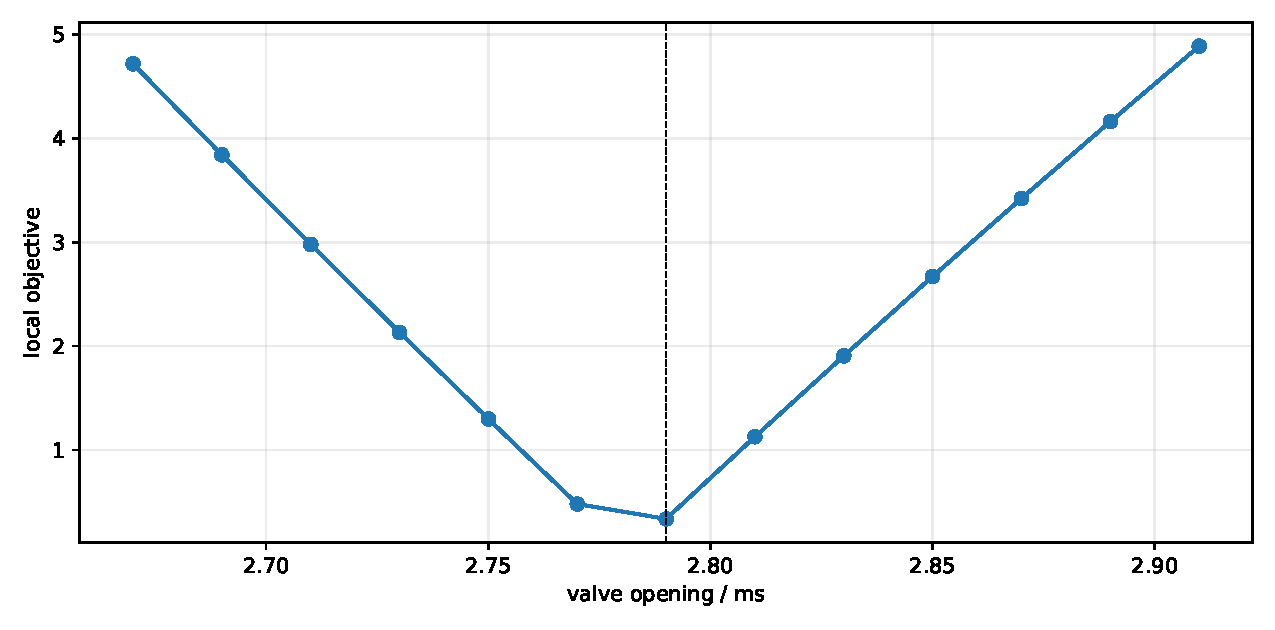
\includegraphics[width=0.86\textwidth]{figures/q1_local_profile.pdf}
\caption{问题一开阀时长的局部目标函数剖面}
\label{fig:q1-local-profile}
\end{figure}

150 MPa稳态的情况类似，但相邻候选的方向相反：6.70 ms的均值为149.991 MPa，6.72 ms上升到150.056 MPa，6.68 ms则为149.924 MPa。这里目标均值已经很接近150 MPa，真正需要保留的是周期纹波仍有1.70 MPa峰峰值。因此在后续过渡控制中，$T_{150}$只负责提供平均供油基准，不把它当成一条无波动的压力曲线。

\subsection{调压过程保留切换前后的状态}

三种调压时间的取值并不是从100 MPa和150 MPa两条独立稳态曲线拼接出来的。对每个切换时刻$t_s$，程序先用前一段开阀时间从100 MPa初始状态推进到$t_s$，再在同一时间步之后切换到$T_{150}$。因此表\ref{tab:q1-ramp}中的“切换压力”和“尾段均值”承担不同职责：前者检验切换事件是否发生在目标附近，后者检验切换后是否仍然保留了合理的周期状态。

2 s方案需要8.12 ms的短时补油，之后降到6.70 ms；5 s方案的初始值为6.72 ms，10 s方案则为6.67 ms。2 s方案切换后的尾段均值为149.950 MPa，并不等于150 MPa稳态表中的149.991 MPa，这是因为它带着切换前的密度和喷油相位进入后段。若将切换后重新初始化为150 MPa，会得到更整齐的数字，却丢失了调压过程本身。

\subsection{问题二：柱塞供油不能被一个平均流量替代}

问题二的候选比较先出现一个容易忽略的现象：角速度附近的均值变化比压力标准差变化更快。10 s回放、末3 s统计下，27.507 rad/s的均值为100.005 MPa，标准差1.124 MPa；把角速度减到27.497 rad/s，均值变为99.960 MPa，RMSE反而略高。于是本问保留均值偏差和RMSE的加权指标，而不是单独追求最小标准差。

\begin{table}[H]
\centering
\caption{问题二角速度局部候选}
\label{tab:q2-local-a}
\small
\begin{tabular}{rrrrrr}
\toprule
$\omega$/(rad/s) & 均值/MPa & 标准差/MPa & RMSE/MPa & 最小/MPa & 最大/MPa\\
\midrule
27.4770 & 99.8774 & 1.1221 & 1.1288 & 97.3036 & 102.4689\\
27.4870 & 99.9182 & 1.1230 & 1.1260 & 97.3160 & 102.4538\\
27.4970 & 99.9598 & 1.1238 & 1.1245 & 97.3321 & 102.4994\\
27.5070 & 100.0046 & 1.1245 & 1.1245 & 97.4235 & 102.5623\\
\bottomrule
\end{tabular}
\end{table}

\begin{figure}[H]
\centering
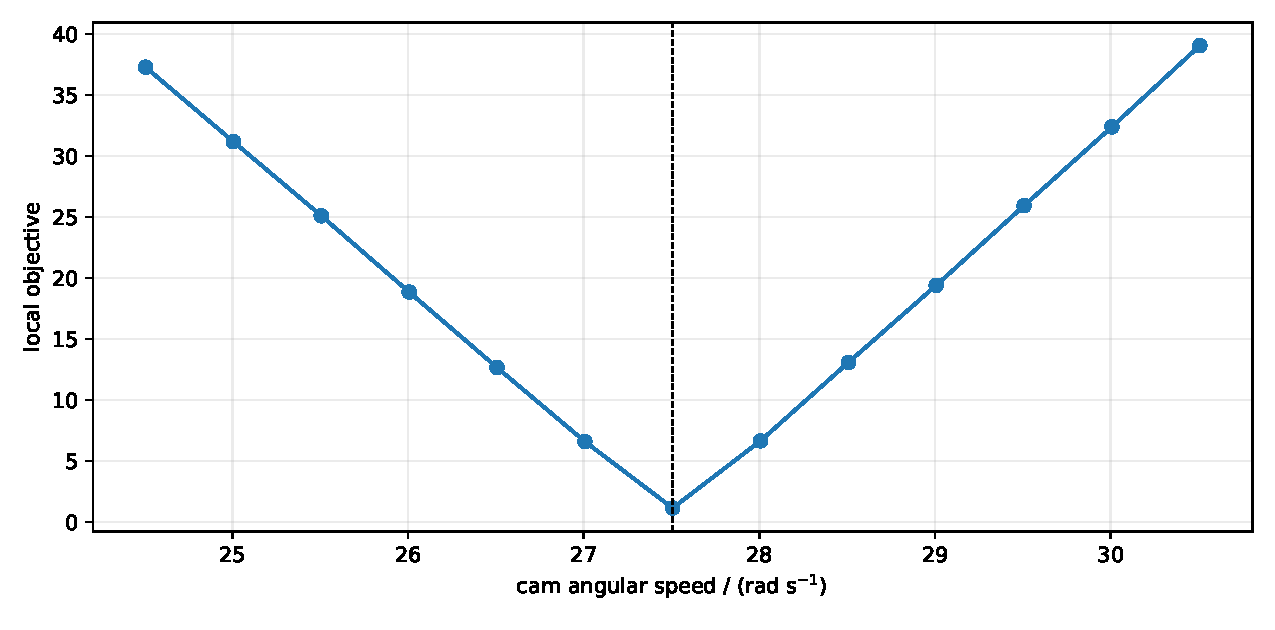
\includegraphics[width=0.86\textwidth]{figures/q2_local_profile.pdf}
\caption{单喷嘴角速度的局部目标函数剖面}
\label{fig:q2-local-profile}
\end{figure}

这组结果使模型选择出现了明确的取舍。若把喷油质量在一个100 ms周期内平均，角速度只会改变平均供油量，无法解释27.49--27.51 rad/s之间的均值和局部峰谷变化；保留凸轮半径和针阀升程的相位后，柱塞供油脉冲与排油脉冲在时间上重新安排，均值和波动才会同时被读出来。这里的“先看波动，再看均值”不是固定写作套语，而是由相邻候选的实际数字迫使我们保留的判断顺序。

\subsection{腔压事件给出了压力曲线的中间层}

管内压力曲线只能告诉我们结果，不能直接说明供油阀为什么在某一个时刻开启。为此，程序把柱塞腔压力和管压同时保存。图\ref{fig:q2-event-window}截取末段250 ms：凸轮压缩时腔压先上升，超过管压后形成供油质量；喷油平台结束后管压回升，腔压与管压的相对次序又使单向阀关闭。供油脉冲因而不是固定贴在凸轮几何上止点，而是被管内当前状态移动。

\begin{figure}[H]
\centering
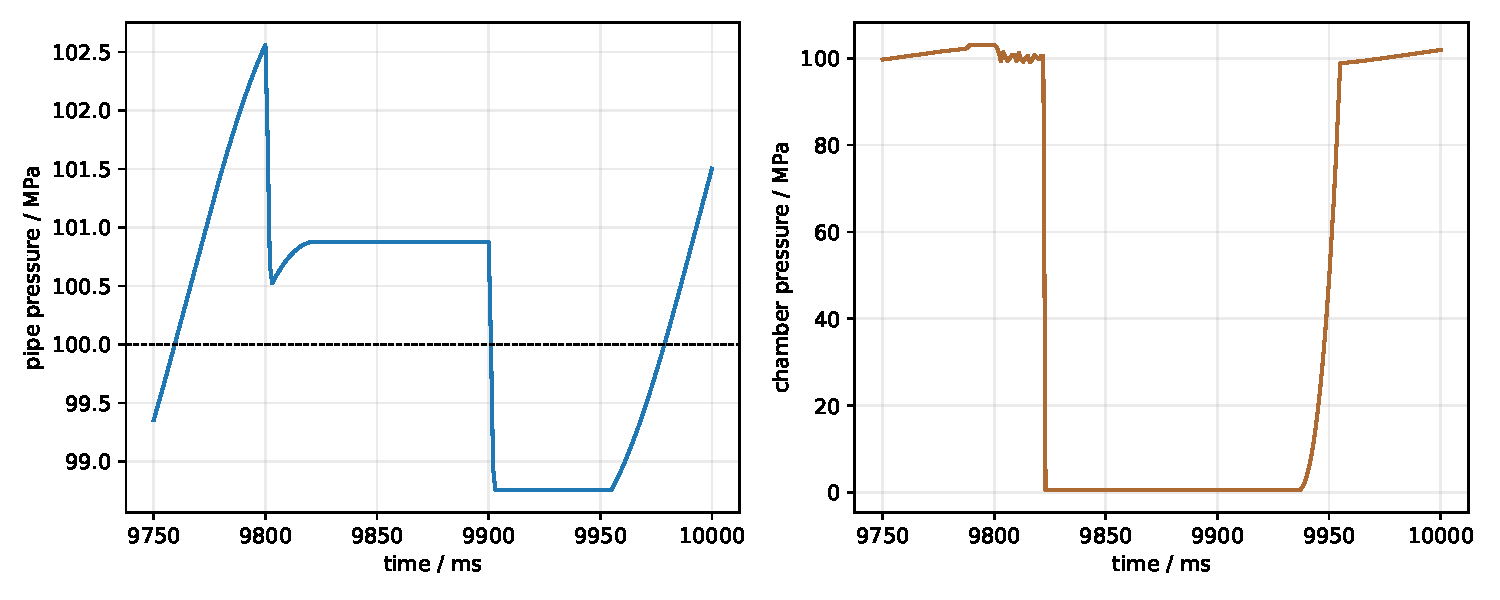
\includegraphics[width=0.96\textwidth]{figures/q2_event_window.pdf}
\caption{问题二末段的管压与柱塞腔压事件窗口}
\label{fig:q2-event-window}
\end{figure}

在问题二的末3 s中，压力落在$[98,102]$ MPa的时间比例为约93.6\%，落在$[99,101]$ MPa的比例约57.8\%，并发生35次穿越100 MPa的事件。这个统计不能替代波形图，却能把“压力大致稳定”具体化：模型不是没有波动，而是大部分时间保持在2 MPa带内，峰谷仍由周期执行机构产生。

\subsection{问题三：相位差的取舍需要看联合搜索}

第二个喷嘴的相位差不能先凭几何直觉固定为50 ms，再去调角速度。本文先用与问题二相同的状态模型做二维搜索，再在候选附近以0.00002 rad/ms和2 ms的网格回放。最终候选为54.717 rad/s、48.052 ms；48.052 ms附近的46.052 ms和50.052 ms分数也接近，因而这里只把48.052 ms视为本次离散回放下的代表性方案。

\begin{figure}[H]
\centering
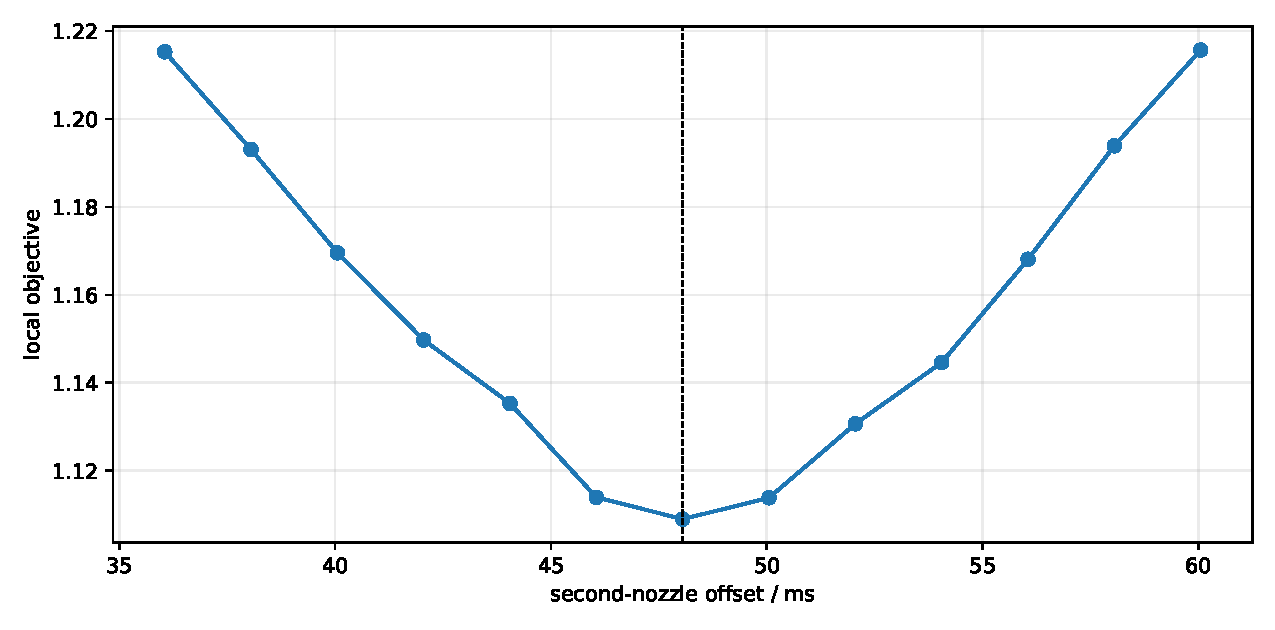
\includegraphics[width=0.86\textwidth]{figures/q3_offset_profile.pdf}
\caption{固定角速度时第二喷嘴相位差的局部剖面}
\label{fig:q3-offset-profile}
\end{figure}

无减压阀时，双喷嘴的均值为100.003 MPa，峰峰值5.018 MPa，末3 s中落入$[98,102]$ MPa的时间比例约94.1\%。相比单喷嘴，双喷嘴并没有把压力波动自动消除；它只是把排油事件变得更密集，使相位差有机会改变局部峰值的位置。相位差应该被看作事件排列的控制量，而不是越接近半周期就一定越优。

\subsection{减压阀的作用由两个指标共同决定}

若减压阀只按最高压力排序，泵速倍率会被压在较低水平，阀门不断排出高压阶段的质量，均值随之向低侧移动。本文把泵速倍率和滞回阈值放在同一有限网格中回放，得到倍率1.12、高阈值101.8 MPa、低阈值101.5 MPa。带阀方案的末3 s均值为99.984 MPa，标准差1.128 MPa，峰峰值4.477 MPa，最高压力101.802 MPa；与无阀方案相比，峰值下降约0.68 MPa，均值只改变约0.019 MPa。

这里的结论不是“减压阀越灵敏越好”。滞回宽度为0.3 MPa时，阀门在阈值附近有明确的开、关区间；若把低阈值抬得太高，阀门打开后迟迟不关，低压谷值会被拉长；若把高阈值压得过低，阀门承担了本应由泵速和相位承担的平均供油任务。正因如此，正文同时报告阈值、泵速倍率、均值和峰峰值，避免用一个“降峰率”掩盖职责错配。

\subsection{三种积分步长的对照}

步长检验不把0.02 ms自动当成真值，而是比较同一控制量在0.08、0.04和0.02 ms下的回放。问题二的末3 s均值分别为99.545、99.407和99.344 MPa，峰峰值分别为5.207、5.212和5.210 MPa；问题三带减压阀的均值分别为99.913、99.945和99.948 MPa，峰峰值分别为4.573、4.515和4.441 MPa。峰峰值变化小于均值的系统性偏移，说明这里的主要差别来自长时相位和离散事件，而不是一个简单的线性积分误差。

\begin{table}[H]
\centering
\caption{三种积分步长下的末段读数}
\label{tab:step-convergence-a}
\small
\begin{tabular}{llrrrr}
\toprule
工况 & $\Delta t$/ms & 均值/MPa & 标准差/MPa & 最小/MPa & 峰峰值/MPa\\
\midrule
问题一 & 0.08 & 100.7078 & 0.0344 & 100.3218 & 0.4984\\
问题一 & 0.04 & 100.3227 & 0.0370 & 99.9703 & 0.3950\\
问题一 & 0.02 & 100.3310 & 0.0376 & 99.9724 & 0.3842\\
问题二 & 0.08 & 100.2302 & 1.1259 & 97.6389 & 5.1399\\
问题二 & 0.04 & 100.0696 & 1.1249 & 97.4890 & 5.1379\\
问题二 & 0.02 & 100.0046 & 1.1245 & 97.4235 & 5.1387\\
双喷嘴+阀 & 0.08 & 99.9897 & 1.1236 & 97.2441 & 4.5752\\
双喷嘴+阀 & 0.04 & 99.9970 & 1.1274 & 97.2540 & 4.5477\\
双喷嘴+阀 & 0.02 & 99.9837 & 1.1280 & 97.3252 & 4.4769\\
\bottomrule
\end{tabular}
\end{table}

\begin{figure}[H]
\centering
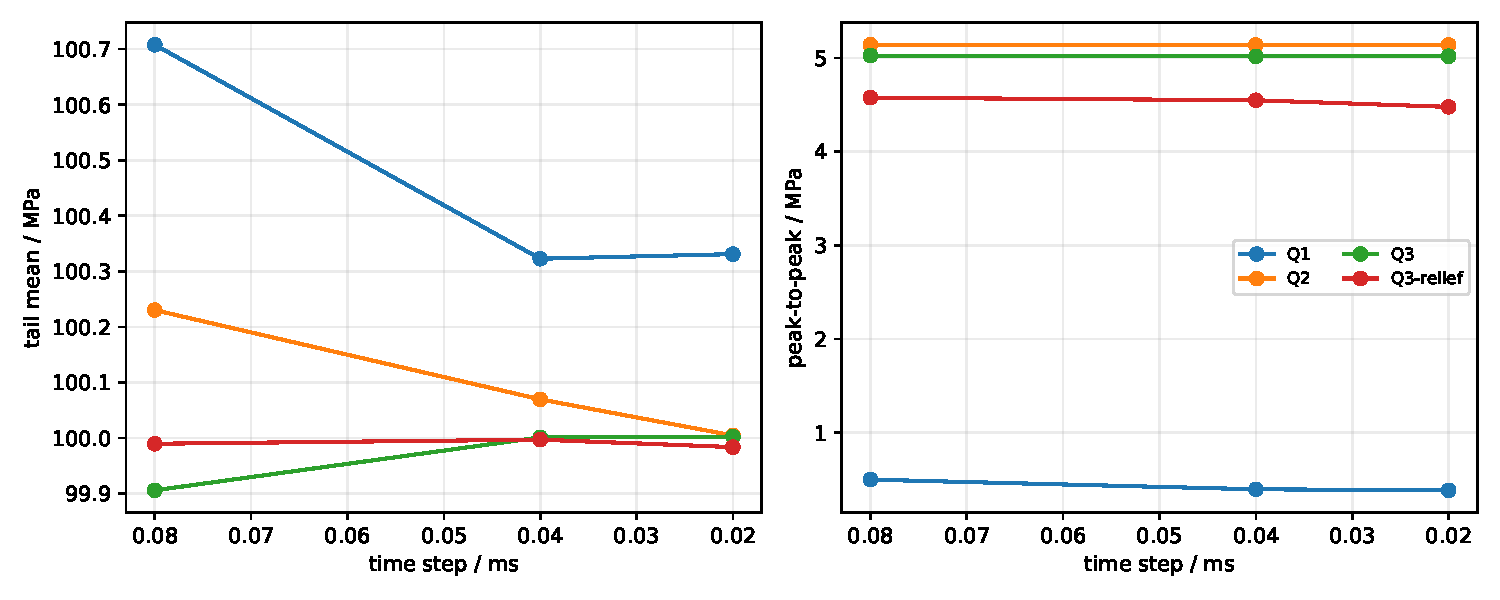
\includegraphics[width=0.96\textwidth]{figures/step_convergence.pdf}
\caption{不同积分步长下的均值和峰峰值对照}
\label{fig:step-convergence-a}
\end{figure}

\subsection{结果解释的范围}

以上复核可以支持三类判断：固定泵压下的开阀时长在离散网格中可复算；凸轮供油的角速度和双喷嘴相位在有限搜索中有一组均值、波动兼顾的候选；减压阀在提高泵速倍率后可以降低峰峰值而不明显改变均值。它们不能支持三类更强的说法：不能据此推断连续参数域的全局最优，不能把题面流量系数视为实物标定值，也不能把单体油管模型推广成具有空间压力波传播的真实管路。

\subsection{公开判断轨迹的复现顺序}

若要复核本文某一个数字，顺序应当是先检查输入表的行数、单位和范围，再检查状态表是否以100 MPa处的0.850 mg/mm$^3$为基准，随后查看候选控制量的局部剖面，最后才读压力曲线。这个顺序比“先看最优值，再补一句模型解释”更能发现问题：若局部剖面已显示候选落在离散跳变处，就不应在文字中使用连续敏感性；若管压和腔压的事件次序不对，单看尾段均值也不能把程序称作稳定。

\begin{table}[H]
\centering
\caption{从输入到结论的公开复核链}
\label{tab:judgement-trace-a}
\small
\begin{tabularx}{\textwidth}{p{2.1cm}p{4.0cm}p{4.1cm}X}
\toprule
复核层 & 先问什么 & 本稿的证据 & 允许写出的结论\\
\midrule
数据 & 记录粒度和单位是否一致 & 三份附件行数、范围及读入接口 & 说明数据在模型中的职责\\
状态 & 质量变化能否回到压力 & 式\eqref{eq:rho}、质量收支、极限检查 & 说明状态转换自洽\\
事件 & 哪个动作先发生 & 单向阀、喷嘴、减压阀的时间步顺序 & 解释局部峰谷和相位\\
候选 & 相邻控制量是否跨步 & 局部剖面和候选表 & 选择离散设置下的代表值\\
结果 & 结论是否依赖回放口径 & 10 s末3 s、步长对照和JSON & 给出有边界的可复算方案\\
\bottomrule
\end{tabularx}
\end{table}

这条复核链也决定了本文的写法：先交代数据怎样进入状态，遇到分叉时写出比较过的候选，结果之后紧跟解释和不能推出的结论。这样保留的是公开的判断依据，而不是把不可检查的内部思维过程包装成论文内容。

\section{数值实现的逐步展开}

前文已经给出了连续形式的质量收支，实际计算还需要回答三个离散问题：压力状态表怎样建立，执行机构在一个时间步内按什么次序更新，以及搜索得到的候选怎样回放。把这三件事分开写，是为了让公式、程序和结果之间有明确的接口。

\subsection{压力状态表的生成与反解}

附件3给出的是$E(P)$而不是直接给出的密度函数。程序先在$P_j=0.01j$ MPa上用线性插值得到$E_j$，再用梯形公式计算
\begin{equation}
 I_{j+1}=I_j+\frac{P_{j+1}-P_j}{2}\left(\frac{1}{E_j}+\frac{1}{E_{j+1}}\right),\qquad I_0=0.
\end{equation}
由此构造
\begin{equation}
 \rho_j=0.850\exp(I_j-I_{100}),
 \qquad P(\rho_j)=\operatorname{interp}(\rho_j;\rho_j,P_j).
\end{equation}
第一式负责把压力查成密度，第二式负责在质量收支之后把密度查回压力。两次插值的网格相同，避免一个分支用压力积分、另一个分支用固定压缩系数。压力网格覆盖0--200 MPa，正好覆盖附件3的原始范围；程序没有用端点外推来制造更宽的适用区间。

这种处理还有一个实际好处：当流量差很小时，状态更新发生在密度上，压力只在需要输出时反解。若直接对压力写显式差分，$E(P)$会出现在分母，并且在压力变化较大的喷油起始段放大步长误差；质量作为中间量则始终有清楚的单位。对任意一步，程序都可以检查$\rho V_p$是否等于上一步质量加入口质量减出口质量，这个检查比只看最终压力更早暴露单位错误。

\subsection{问题一的一个时间步}

问题一的状态更新按以下次序执行。设当前时刻为$t_k$，周期相位为$\tau_k=t_k\bmod100$ ms。先由$\tau_k<T_v$判断入口阀，再由式\eqref{eq:spray}得到喷油体积流量，随后把入口和出口都换成质量流率，最后更新密度并反解压力。

\begin{table}[H]
\centering
\caption{问题一单个时间步的执行接口}
\label{tab:q1-step-a}
\small
\begin{tabularx}{\textwidth}{p{1.3cm}p{4.0cm}p{4.2cm}X}
\toprule
步序 & 读取量 & 分支或计算 & 写出量\\
\midrule
1 & $t_k,T_v$ & 计算$\tau_k$并判断入口阀开闭 & $I_v(t_k)$\\
2 & $\tau_k,P_k$ & 按分段喷油曲线求$q_o$，再乘$\rho(P_k)$ & $\dot m_o$\\
3 & $P_k,I_v$ & 按160 MPa入口压差求孔口质量流率 & $\dot m_i$\\
4 & $\dot m_i,\dot m_o,V_p$ & 用显式质量收支更新密度 & $\rho_{k+1}$\\
5 & $\rho_{k+1}$ & 在状态表中反解压力 & $P_{k+1}$\\
\bottomrule
\end{tabularx}
\end{table}

表\ref{tab:q1-step-a}中的次序不能随意交换。例如先用$P_{k+1}$判断入口阀会把同一时间步的入口流量重复计算；先把喷油速率取周期平均，又会把2.4 ms喷油窗口的上升、平台和下降压成一个常数。本文的程序只有一个质量更新位置，入口、喷油和减压项都在这里汇合，因此可以把一张压力表对应回一次完整的质量增减。

\subsection{问题二的腔体事件}

问题二增加了一个随相位变化的柱塞腔。令上一时刻腔体积为$V_{c,k-1}$，当前体积为$V_{c,k}$。当$V_{c,k}>V_{c,k-1}$时，程序按题面把低压油重新补入腔体；当$V_{c,k}\leq V_{c,k-1}$时，腔内质量保持，腔压由当前体积和质量共同决定。只有$P_{c,k}>P_k$时，单向阀质量流率才非零。这样处理后，问题二的“供油”是压力事件，不是预先写死的开阀占空比。

\begin{equation}
 P_{c,k}=\rho^{-1}\left(\frac{m_{c,k}}{V_{c,k}}\right),\qquad
 \dot m_{c,k}=\begin{cases}
 \rho(P_{c,k})CA_i\sqrt{2(P_{c,k}-P_k)/\rho(P_{c,k})},&P_{c,k}>P_k,\\
 0,&P_{c,k}\leq P_k.
 \end{cases}
\end{equation}

腔体补液和向油管供油是两个相反方向的动作。若只在第一周期把腔体初始化为0.5 MPa，后续周期会因为质量未补足而逐渐变成“空腔”；若在所有相位都强行补足，压缩段的供油质量又会被凭空增加。本文把体积增大作为补液触发条件，把压力比较作为单向阀触发条件，二者分别对应几何变化和流向变化。

\subsection{问题三的状态码与动作顺序}

问题三包含两个喷嘴和一个减压阀。一个时间步内先由凸轮相位决定柱塞体积，再由两个喷嘴相位计算排油，随后比较腔压和管压决定泵侧质量，最后依据减压阀的滞回状态决定是否排出额外质量。程序中的减压状态只有0和1：当管压达到$P_H$时置1，降到$P_L$时置0，位于两者之间时保持上一状态。

\begin{table}[H]
\centering
\caption{问题三一个时间步的状态码更新}
\label{tab:q3-state-code-a}
\small
\begin{tabularx}{\textwidth}{p{1.4cm}p{4.0cm}p{4.0cm}X}
\toprule
状态码 & 触发条件 & 本步动作 & 传给下一步的状态\\
\midrule
0 & $P<P_H$且上一步关闭 & 不产生减压质量流率 & 保持0，除非达到$P_H$\\
1 & $P\geq P_H$或此前已开启 & 按孔口式排出减压质量 & 保持1，直到$P\leq P_L$\\
切换 & $P_H$或$P_L$被跨越 & 只在当前步改变一次状态 & 下一步使用新状态\\
\bottomrule
\end{tabularx}
\end{table}

把状态码写出来以后，减压阀的作用就不会被误写成“把压力整体向下平移”。它只在高压区间排油，排出的质量会改变下一时间步的管压和柱塞供油条件；泵速倍率之所以需要重新搜索，正是因为阀门改变了质量收支而不是只改变一个输出显示值。

\subsection{搜索范围、候选数量与最终回放}

所有搜索都分成定位和裁决两步。定位阶段的目标是找到可能的量级，裁决阶段则统一使用最终回放的时间长度和统计窗口。表\ref{tab:search-contract-a}列出了实际范围；“步长”是搜索变量的网格步长，不是积分步长。

\begin{table}[H]
\centering
\caption{三问搜索合同}
\label{tab:search-contract-a}
\small
\begin{tabularx}{\textwidth}{p{1.9cm}p{3.7cm}p{3.4cm}p{3.5cm}X}
\toprule
问题 & 定位方式 & 最终变量步长 & 回放与评分窗口 & 取舍依据\\
\midrule
问题一 & 标量粗区间和二分 & 0.02 ms & 20 s，末5 s & 均值偏差加标准差，并查看相邻步\\
问题二 & 固定种子差分进化 & $0.00001$ rad/ms & 10 s，末3 s & RMSE加两倍均值偏差\\
问题三 & 一致口径二维差分进化 & $0.00002$ rad/ms、2 ms & 10 s，末3 s & 联合考虑均值、纹波和相位\\
减压阀 & 有限网格枚举 & 倍率、阈值、滞回宽度 & 同上 & 最高压力不能牺牲平均供油\\
\bottomrule
\end{tabularx}
\end{table}

这里的“合同”是为了限制文字对数值的追随。如果先得到一组数字，再任意改变尾段窗口直到数字好看，搜索就失去了可比性。本文的候选剖面和步长表使用与正式结果相同的回放口径；如果更换回放长度，必须重新生成摘要、结果表和图，而不能只改一处小数。

\section{输出量的解释与同步}

\subsection{均值、波动和极值各自回答一个问题}

均值回答的是长期质量收支是否平衡，标准差回答的是周期纹波大小，最小值和最大值则回答某一次喷油或阀门事件是否越过安全边界。三个量不能互相代替。问题二的均值几乎为100 MPa，但最小值仍为97.424 MPa；问题三带减压阀的最大值压到101.802 MPa，最低值却仍有97.325 MPa。若把均值作为唯一结果，读者会看不见减压阀对上、下两侧的不同作用。

为便于复核，诊断文件还记录了目标穿越次数和落入压力带的比例。单喷嘴末3 s穿越100 MPa 35次，双喷嘴74次，带减压阀87次；带阀后落入$[98,102]$ MPa的比例达到94.8\%，但落入$[99,101]$ MPa的比例只有60.7\%。这两个比例同时说明：减压阀改善了宽压力带内的可接受性，却没有把周期波动消除成一条直线。

\subsection{图形不是结果表的装饰}

图\ref{fig:q1-control}用于看调压过程是否连续，图\ref{fig:q23-pressure}用于比较执行机构层次，图\ref{fig:q2-event-window}用于追踪腔压事件，图\ref{fig:step-convergence-a}用于判断积分步长是否改变结论方向。四类图形各有职责，因此没有把所有曲线压进一张“总结果图”。局部剖面图则承担另一项任务：它们显示相邻候选的相对位置，帮助判断某个控制量的末位是否有物理意义。

\subsection{结果文件的单向数据流}

正式运行时，输入只从三个Excel附件进入\path{load_inputs}；状态表由\path{state_table}生成；三问结果由\path{q1_analysis}和\path{q2_q3_analysis}写入\path{summary.json}；诊断脚本再读取该JSON和同一批附件，生成CSV剖面、步长表和\path{diagnostics.json}。正文的表格和图形只引用这些输出，不在TeX中重新计算压力。

\begin{table}[H]
\centering
\caption{结果文件之间的单向依赖}
\label{tab:result-flow-a}
\small
\begin{tabularx}{\textwidth}{p{3.2cm}p{3.8cm}p{4.0cm}X}
\toprule
文件或目录 & 上游 & 写出的信息 & 正文接口\\
\midrule
\path{data/*.xlsx} & 官方附件 & 三组原始数组 & 表\ref{tab:input-audit-a}\\
\path{summary.json} & 主求解器和固定种子 & 控制量、压力统计、搜索边界 & 表\ref{tab:all-results-a}\\
\path{diagnostics.json} & summary、附件和诊断脚本 & 局部候选、事件比例、步长对照 & 表\ref{tab:step-convergence-a}\\
\path{figures/*.pdf} & 两个Python脚本 & 状态图、控制曲线、剖面图 & 各结果图\\
\path{formal.tex} & 上述输出的人工编排 & 解释、边界和引用 & 本文\\
\bottomrule
\end{tabularx}
\end{table}

单向数据流的意义在于，若新运行改变了问题三的相位差，影响会沿着JSON、诊断表、图形、结果表和摘要逐层显现；若某个文件没有更新时间变化，便可以在提交前定位到同步遗漏，而不是靠肉眼在长文中寻找旧数字。

\section{替代简化方案的排除}

建模时并不是模型越复杂越好，关键在于一个简化是否删掉了题目真正要求观察的事件。本节把计算中考虑过、但没有作为正式方案使用的三种简化列出来。它们的共同点是看起来可以减少代码或缩短篇幅，实际却会使某个问题失去可解释的中间量。

\subsection{不把喷油曲线换成周期平均量}

由式\eqref{eq:spray}积分可得单个喷嘴一个周期的排油体积为
\begin{equation}
 \int_0^{100}q_o(\tau)\dd\tau
 =\frac{1}{2}\times0.2\times20+2.0\times20
 +\frac{1}{2}\times0.2\times20=44\ \mathrm{mm^3},
 \qquad \overline q_o=0.44\ \mathrm{mm^3/ms}.
\end{equation}
若把它直接代替分段曲线，平均质量收支仍然可能接近，但喷油开始的下降段会被摊到整个100 ms周期，压力峰谷的时间位置就不再对应针阀事件。问题一的调压切换、问题二的腔压越过管压、问题三的两喷嘴相位都依赖这个时间位置，因此本文只在结果解释中使用平均流量作数量级检查，没有把它写进主仿真。

\subsection{不把单向阀和减压阀合并成一个开关}

单向阀的触发条件是$P_c>P$，它决定燃油从柱塞腔流入油管；减压阀的触发条件是$P\geq P_H$或$P\leq P_L$，它把油管中的燃油排向低压侧。两个阀门的流向、位置和状态变量都不同。如果把它们合成一个“压力高就加、压力低就减”的开关，柱塞腔质量会被错误地当成油管质量的一部分，且无法解释图\ref{fig:q2-event-window}中的腔压先于管压变化。

\begin{table}[H]
\centering
\caption{三种替代简化及其被排除的原因}
\label{tab:excluded-simplifications-a}
\small
\begin{tabularx}{\textwidth}{p{3.1cm}p{3.7cm}p{4.4cm}X}
\toprule
简化方案 & 保留下来的量 & 被删掉的事件 & 本文的处理\\
\midrule
周期平均喷油 & 一个周期排油体积44 mm$^3$ & 上升沿、平台和下降沿的时刻 & 保留式\eqref{eq:spray}的分段曲线\\
单一压力开关 & 管内压力$P$ & 腔压、管压和两个阀门的不同流向 & 分别更新单向阀和减压阀\\
一个总评分 & 一个综合数值 & 均值、峰值和低侧谷值的职责差异 & 同时报均值、标准差、极值和峰峰值\\
\bottomrule
\end{tabularx}
\end{table}

\subsection{不把所有结果压成一个总分}

问题一固定压力泵的标准差只有0.038 MPa，问题二和问题三的标准差约1.1 MPa；但如果只比较RMSE，问题一会自然占优，无法回答题面中“柱塞和双喷嘴怎样调整”的问题。另一方面，减压阀把峰峰值从5.018 MPa降至4.477 MPa，却伴随泵速倍率增大和阈值上移。若只比较最大压力，阀门可能被调得过于频繁；若只比较均值，阀门的限压职责又完全看不出来。因此本文使用加权目标完成搜索，使用多项原始统计完成解释，搜索指标和论文结论不承担同一个职责。

这些被排除的简化也给后续改进留下了清楚的入口：若有实测喷油曲线，可以替换式\eqref{eq:spray}而不改质量状态；若有阀门响应时间，可以在状态码1和0之间增加延迟；若比赛题目明确给出多目标权重，则可将均值、峰值和波动写成外层决策，而不是事后凭一句“综合考虑”带过。

\section{模型评价与改进}

\subsection{模型能解释什么}

分层状态模型把题面的三类信息放在了不同位置：附件3只改变状态转换，附件1改变柱塞腔容积，附件2改变喷孔有效面积，阀门和减压器则通过事件逻辑进入质量收支。这样可以解释为什么同样是100 MPa附近，固定压力泵的波动远小于柱塞供油的波动，也可以解释为什么减压阀降低峰值的同时会拉低均值。

模型还保留了几个可直接回查的量：100 MPa时的燃油密度为0.850 mg/mm$^3$，油管体积为39269.908 mm$^3$，入口孔面积和喷孔面积均由题面直径计算，喷油曲线的持续区间为2.4 ms。它们不依赖求解器的名称，换成另一种积分器后仍可以作为接口检查。

\subsection{模型不能支持的结论}

首先，压力只在油管内被视为均匀，不能解释入口到喷嘴之间的传播延迟和空间压力波。其次，流量系数、低压侧压力和针阀升程均按题面或附件直接使用，没有独立实验标定。再次，差分进化和局部网格的结果依赖搜索范围、种子和步长；它们只证明当前候选在回放中较好，不证明连续控制域的全局最优。最后，减压阀的机械响应时间没有给出，滞回模型是一个可复算的控制近似，不是实物阀门的完整动力学。

\subsection{可执行的改进方向}

若能取得实测压力曲线，第一步应把流量系数和针阀升程的时间延迟作为待标定参数，并用同一组压力窗口同时校准均值和相位。第二步可以把油管离散成多个控制体，检查压力波传播是否会改变两个喷嘴的最佳相位。第三步在减压阀中加入最小开闭时间和响应延迟，再比较滞回宽度对谷值和峰值的影响。上述改进都对应当前模型已指出的一个具体缺口；本稿没有把它们写成已经完成的实验。

\subsection{误差预算与独立数量级复算}

本文不能给出统计意义上的置信区间，因为题面没有提供重复实验压力序列；但可以把结果的不确定来源分层记录。附件和模型假设决定“是否描述了真实装置”，状态插值与时间步长决定“同一模型是否算得稳定”，控制量网格和随机定位决定“候选是否被搜索过程遗漏”。这几类误差不能简单相加，也不能用一次步长对照替代实验误差。

\begin{table}[H]
\centering
\caption{本模型的误差预算与已完成检查}
\label{tab:error-budget-a}
\small
\begin{tabularx}{\textwidth}{p{2.4cm}p{3.8cm}p{4.7cm}X}
\toprule
误差层 & 来源 & 本次可见影响 & 结论中的处理\\
\midrule
数据与结构 & 凸轮、针阀和弹性模量附件；油管均匀压强假设 & 无实测压力可用于外部标定，空间压力波未建模 & 不声称实物控制精度\\
状态插值 & $E(P)$线性插值、0.01 MPa压力网格 & 状态表输出粒度有限，表外规律未验证 & 结果保留到与网格相称的小数位\\
时间推进 & 显式更新与阀门事件离散 & 0.04降至0.02 ms时，问题一均值变化0.0083 MPa，问题二变化0.0650 MPa & 报告步长并给出对照表\\
控制量网格 & 开阀时长、角速度和相位的局部步长 & 2.77与2.79 ms使均值相差0.805 MPa；27.497与27.507 rad/s使均值相差0.0449 MPa & 把相邻候选写入正文，不解释虚假末位\\
搜索定位 & 固定种子差分进化后再局部网格 & 粗值只确定邻域，正式参数来自一致口径回放 & 只称离散候选，不称连续全局最优\\
\bottomrule
\end{tabularx}
\end{table}

另做一个不依赖优化器的数量级检查。油管体积为39269.908 mm$^3$，100 MPa处密度为0.850 mg/mm$^3$，故管内燃油质量约为33379.42 mg；单个喷嘴每周期排油44 mm$^3$，按同一密度估算约37.4 mg，只占管内总质量的$1.12\times10^{-3}$。因此一次喷油造成的是有限幅度的周期波动，而压力均值需要由许多周期的净质量差逐步调整。这个数量级与问题一短时调压需要提高开阀时长、问题二和三需用长时尾段裁决的现象一致；若程序一次喷油便把管压推到附件范围之外，应先检查单位和质量收支，而不是继续调优化参数。

\section{结论}

本文由压力--密度积分关系和燃油质量守恒出发，完成了三个层次的控制计算。固定160 MPa泵压下，100 MPa保持的单周期阀门开启时长为2.7900 ms，150 MPa保持时为6.7000 ms；2 s、5 s、10 s调压过程的初始开启时长分别为8.1200、6.7200、6.6701 ms。凸轮柱塞和单喷嘴模型给出27.507 rad/s的角速度候选，末3 s均值100.005 MPa。双喷嘴模型给出54.717 rad/s和48.052 ms相位偏移；在此基础上设置减压阀高、低阈值101.8/101.5 MPa并将泵速倍率调为1.12，最高压力约101.80 MPa，平均压力约99.98 MPa。上述参数是10 s回放和0.02 ms积分设置下的可行解，不能替代连续参数域的全局证明。

结果的主要含义不是某个控制数值的绝对精确，而是三个控制量的职责可以分开：阀门开启时长决定平均补油量，凸轮角速度和喷嘴相位决定周期结构，减压阀负责处理上冲而会同时带来低侧损失。所有数值均以附件数据、固定时间步长和有限搜索为前提；在没有实测压力和阀门响应参数时，结论应作为题面条件下的可复算控制方案。
\label{mcm-body-end}

\begin{thebibliography}{9}
\bibitem{problem2019a} 2019 高教社杯全国大学生数学建模竞赛 A 题：高压油管的压力控制，官方题面及附件1--3。
\bibitem{solver2019a} 本文独立求解器输出：\path{analysis/model_pipeline.py}及\path{analysis/results/summary.json}，运行日期2026-08-14。
\end{thebibliography}

\appendix
\section{算法执行清单}
正文中的公式对应如下执行动作：先读入三个附件并检查空行；再在0--200 MPa上插值弹性模量并积分得到密度；问题一先用粗步长定位，再以0.02 ms候选网格和20 s回放比较相邻开阀步数；问题二先以固定种子定位角速度，再以10 s回放、末3 s指标做0.00001 rad/ms细化；问题三先做一致口径的二维搜索，再以0.00002 rad/ms和2 ms的局部网格细化，减压阀在同一回放口径下枚举泵速倍率和滞回阈值；最后把数组结果写入JSON并生成八张PDF图。完整循环保留在\path{analysis/model_pipeline.py}和\path{analysis/diagnostics.py}中，附录只列接口，避免把数百行代码复制成无法核对的长表。

\begin{longtable}{p{3.2cm}p{5.3cm}p{6.2cm}}
\caption{状态更新接口}\label{tab:algorithm-a}\\
\toprule
阶段 & 读取 & 写出\\
\midrule
状态表 & 附件3压力、弹性模量 & 压力网格、密度网格、模量网格\\
问题一 & 阀门开度、喷油相位、管内密度 & 管内压力序列、尾段指标和相邻候选\\
问题二 & 凸轮半径、针阀升程、角速度 & 腔压、管压、单向阀事件和局部剖面\\
问题三 & 两个喷嘴相位、减压阈值、泵速倍率 & 减压状态、双喷嘴压力序列和步长对照\\
复现 & JSON、CSV、图形和脚本哈希 & 正文数字、表格和图形接口\\
\bottomrule
\end{longtable}

\section{离散步长和结论强度}
本次积分使用0.02 ms步长，图形保存间隔为1 ms；搜索阶段使用更粗步长只承担候选定位，最终读数来自细步长回放。步长越小并不自动等于模型更正确，因为附件曲线本身是离散表格，压力--密度关系也是插值近似。若后续获得实测曲线，应把步长收敛和参数标定作为独立检验，而不能用本次一次回放替代。
\end{document}
